\documentclass[a4paper]{article} % A4 paper and 11pt font size

\usepackage{braket}
\usepackage{amsmath}
\usepackage{amssymb}
\usepackage{bm}
\usepackage[utf8]{inputenc}
\usepackage{verbatim}
\usepackage{tikz}
%\usepackage{pgfornament}
\usepackage{pgfplots}
\usepackage{pgffor}
\usepackage[version-1-compatibility]{siunitx}
\usepackage{fancyhdr}
\usepackage{lipsum}
\usepackage{gensymb}
\usepackage{framed}
\usepackage{cancel}
\usepackage{slashed}
\usepackage{hyperref}
\usepackage{pdflscape}
\usepackage{graphicx}
\usepackage{caption}
\usepackage{subcaption}
\usepackage{geometry}
\usepackage{yfonts}
\usepackage{calc}
\usepackage{cite}
\usepackage{siunitx}


\setlength{\parindent}{0em}
\setlength{\parskip}{1em}
\newcommand{\goth}[1]{{\Huge\textfrak{#1}}}
\renewcommand{\baselinestretch}{1.1}

 \geometry{
 a4paper,
 total={210mm,297mm},
 left=28mm,
 right=28mm,
 top=30mm,
 bottom=40mm,
 }


%----------------------------------------------------------------------------------------
%	TITLE SECTION
%----------------------------------------------------------------------------------------
%\setlength\parindent{0pt} % Removes all indentation from paragraphs - comment this line for an assignment with lots of text

\setcounter{section}{-1}
\pagenumbering{arabic}
\begin{document}
\pagestyle{empty}

\newcommand{\HRule}{\rule{\linewidth}{0.5mm}}

\begin{titlepage}

    \begin{center}
        \textsc{\large SN: 587623}\\[6cm]

        \HRule \\[0.5cm]
		\Huge \textbf{PHYC30019 Astrophysics}\\[0.5cm]
        \huge \textbf{Course Summary}\\[0.5cm] 
        \HRule \\[1.5cm]
        \begin{minipage}{0.4\textwidth}
        \begin{center}

        \large By \\[0.75cm]
        \huge Braden \scshape Moore \\[0.5cm]
        \normalsize \normalfont Master of Science \\
        The University of Melbourne \\

        \end{center}
        \end{minipage}

        \vfill

        \large \today
    \end{center}


\newpage
\end{titlepage}
%----------------------------------------------------------------------------------------
\pagestyle{empty}
%\tableofcontents
%\newpage

\pagestyle{fancy}
\pagenumbering{arabic}
\rfoot{\textsc{Braden Moore, 587623}}
\lfoot{\textsc{\today}}
\lhead{\textsc{Semester 1, 2016}}
\rhead{\textsc{PHYC30019 Astrophysics}}
\setcounter{page}{1}
\section{Introduction}
\subsection{Housekeeping}
\subsubsection{Texts and References}
\begin{itemize}
\item Maoz - Astrophysics in a Nutshell (free download apparently)
\end{itemize}
\subsubsection{Marking system}
\begin{itemize}
\item $3 \times 10\%$ workshops Weeks 4, 8 and 11
\item 70\% exam
\end{itemize}

\subsection{Definitions}
\subsubsection{Astronomy}
\begin{itemize}
\item Colects photons
\item Some branches (small at current) investigates cosmic rays
\item Some investigate gravitational waves
\item Measured quantities for photons:
\begin{itemize}
\item 2 anguar dimensions
\item Spectrum
\item Luminosity (distance)
\item Flux (amount)
\end{itemize}
\item Objects investigated:
\begin{itemize}
\item Planets, asteroids, comets (not investigated in class
\item stars, globular clusters, galaxies, gas clouds,
clusters of galaxies, superclusters, active galactic nuclei
\end{itemize}
\end{itemize}

\subsubsection{Astrophysics}
\begin{itemize}
\item Applies physics and mathematics to understand the universe and its components (formation, structure, evolution, dstribution)
\item Uses many branches of physics and maths
\item Often things are measured imprecisely (order of magnitude)
\item Computational processes are used (some high precision measurements are taken, e.g. for pulsars)
\item Types of radiation processes:
\begin{itemize}
\item thermal (emijng a blackbody), synchrotron,
bremsstrahlung, Compton, inverse Compton
\end{itemize}
\end{itemize}

\subsection{Photons}
\begin{itemize}
\item Can be defined by frequency $c=\lambda\nu$
\item Or energy $E=h\nu$
\item Or temperature $E=kT$
\end{itemize}

\begin{figure}[h]
\centering
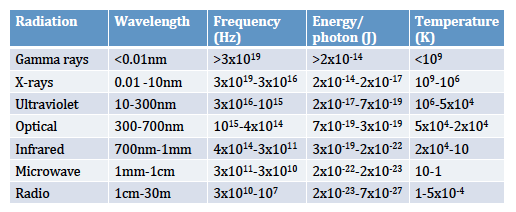
\includegraphics[width=0.7\textwidth]{images/radiation-numbers.png}
\end{figure}

\begin{itemize}
\item Some wavelengths have more attenuation (decay) than others (see figure below)
\end{itemize}

\begin{figure}[h]
\centering
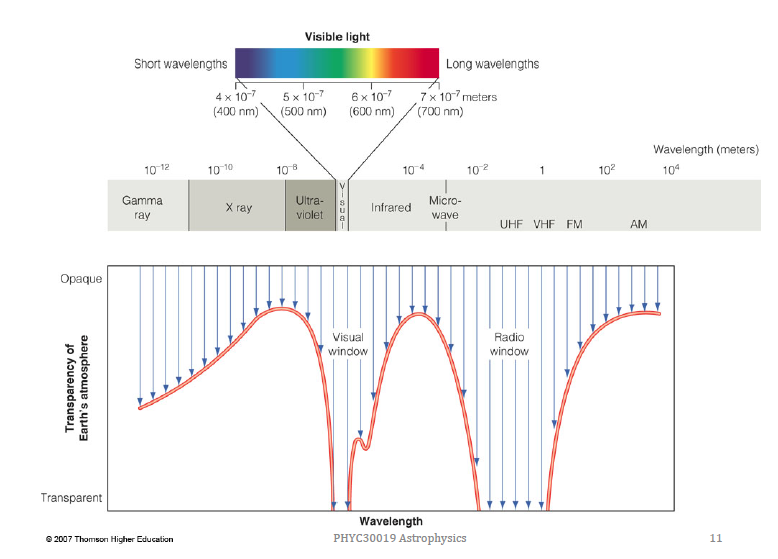
\includegraphics[width=0.7\textwidth]{images/attenuation.png}
\end{figure}


\subsubsection{Characteristic scales}
\begin{itemize}
\item Cosmological
\begin{itemize}
\item Scale of observable universe (light travelling over fininte universe lifetime) $~c/H_0$
\item $H_0$ is Hubble constant
\end{itemize}
\item Parsec
\begin{itemize}
\item $1\text{pc}=3.1\times 10^{18}\text{cm}=3.3\text{ly}$
\item Defined based on universe size
\item Distance at which 1AU (distance to Sun) substends by an angle of one arcsecond
\end{itemize}
\end{itemize}

\subsubsection{Copernican Principle}
\begin{itemize}
\item We are not in a favoured position in the universe.
\item Local physics is the same as distant physics
\item Thus we rarely use "new" physics; exceptions are dark mater and dark energy
\end{itemize}

\subsubsection{Cosmological Principle}
\begin{itemize}
\item On average, the universe is homogeneous and isotropic at any time in its evolution
\item Local measurements of isotropy and homogeny + Coperican principle imply the Cosmological principle
\item Universe is homogenous to about 1\% on a scale of $~100$Mpc
\item We need to average over a large area to get this homogeny
\item Isotropic = rotational invariant
\end{itemize}

\subsection{Astronomical Observing}
Four important dimensions to measure:
\subsubsection{Angular resolution}
\begin{itemize}
\item Smallest angle on the sky between two sources that telescopes can separate
\item Point source produces diffraction pattern with central spot of radius $\theta=1.22\lambda/D$
\item $D=$diameter of aperture (known as Airy disk)
\end{itemize}

\begin{figure}[h]
\centering
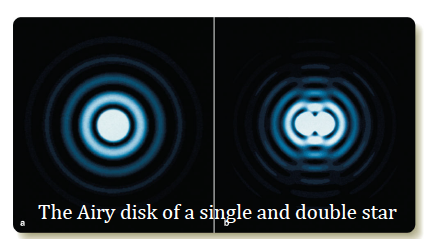
\includegraphics[width=0.6\textwidth]{images/airy.png}
\end{figure}

\subsubsection{Ligth-gathering power}
\begin{itemize}
\item Larger area = more photons collected
\item ILimited by ability to make large glass that doesn't deform
\end{itemize}

\subsection{Integration time}
\begin{itemize}
\item More sensitive if more pghotons are collected
\item Hence, observe for longer
\item Try to have minimal noise
\end{itemize}

\subsubsection{Wavelength range}
\begin{itemize}
\item Different telescopes observe different wavelengths
\item Not all photons reach the Earth, so we have outer space telescopes
\end{itemize}

\subsection{The Big Questions}
\begin{itemize}
\item How did the universe begin and how will it evolve? – the behaviour of matter, energy, space and time
\item What is the nature of the stuff the universe is made of?
\item Physics in extreme physical environments: how does matter behave?
\item How did the universe we inhabit form - stars, galaxies and planets?
\item Are we alone: what do other planetary systems look like? i what is life?
\end{itemize}

\newpage
\section{Blackbody Emission}
\begin{itemize}
\item We approximate a lot of things as blackbodies
\item We assume we can model things by blackbody spectrums
\end{itemize}
\begin{equation}
u_\nu=\frac{8\pi\nu^2}{c^3}\frac{h\nu}{e^{h\nu/kT}-1}
\end{equation}
\begin{itemize}
\item The blackbody spectrum is the energy density $u_\nu$
\item Units: erg cm$^{-3]}$ Hz$^{-1}$.
\item Flow of energy $I_\nu$; derivative of the energy density w.r.t solid angle and multiplying by c
\item = energy passing through unit area per unit time
\end{itemize}
\begin{align}
I_\nu&=c\frac{du_\nu}{d\Omega}=c\frac{u_\nu}{4\pi}\\
&=\frac{2h\nu^3}{c^2}\frac{1}{e^{h\nu/kT}-1}\\
&=B_\nu
\end{align}
\begin{itemize}
\item Called $B_\nu$ because blackbody
\item Flow of energy in a particular direction inside a BB is the intensity $I_\nu$
\item Related to outgoing flux by $df_\nu = I_\nu\cos\theta d\Omega$
\end{itemize}
Okay, I'll just try to summarize stuff as I go along. Very little on written on the board, at the moment.

\begin{itemize}
\item Flux we observe depends on luminosity and distance from star ($f_\nu=\frac{L_\nu}{4\pi ^2}$)
\item Luminosity given by $L_\lambda d\lambda=4\pi^2 R^2 B_\lambda d\lambda$
\item Inverse square law:
\end{itemize}
\begin{equation}
\frac{f_1}{f_2}=\frac{d_2^2}{d_1^2}
\end{equation}

\subsection{Limiting Blackbody Spectra}
At low frequencies,
\begin{align*}
h\nu&\approx kT\\
B_\nu &\sim \frac{2\nu^2}{c^2}kT
\end{align*}

At high frequencies,
\begin{align*}
h\nu&\approx kT\\
B_\nu &\sim e^{-(h\nu/kT)}
\end{align*}


\section{Stars: Observations}
\subsection{Stellar Attributes}
\begin{itemize}
\item Distance
\item Temperatures
\item Luminosity
\item Radius
\item Mass
\end{itemize}

\subsection{Distance}
Parallex, arcsecond, parsec.\\
The Moon is 30 arcminutes across.\\
Distance from Earth to Sun = 1AU.
\begin{equation}
d=\frac{1AU}{\tan(\alpha)}\approx\alpha^{-1}AU
\end{equation}
For small angles (and most stars have very small angles to us) we can use the small angle approximation
\begin{equation}
\tan\theta=\theta+O(\theta^3)
\end{equation}

\subsection{Temperature}
Photon random walks its way out of a star (interacting with electrons). Could take $\sim$3 seconds to get out straight, but actually takes thousands of years.\\
The photosphere is the point where star density is low so a photon can escape without interacting. This is the ``surface".
\subsubsection{Brightness temperature}
Temperature measured at a particular frequency (equivalent temperature for a BB to generate that frequency)
\subsubsection{Colour temperature}
Planck spectrum is fitted to spectrum.\\
The colour of a star is the ratio of two different wavebands.
\subsubsection{Effective temperature}
By using
\begin{equation}
L=4\pi r^2\sigma T^4
\end{equation}
We can measure luminosity, if we know the radius we can find temperature.

\subsection{Magnitudes}
Definition of apparent magnitude:
\begin{equation}
m_\lambda=-2.5\log_{10}f_\lambda+C
\end{equation}
Mimics the human eye (which views things logarithmically). Colours are defined as the difference between magnitudes. UBV system = Ultraviolet, Blue, Visual.\\
\begin{equation}
B-V=m_B-m_V
\end{equation}
More B = bluer. NOTE: independent of distances (they cancel out b/c logarithic difference).

\subsection{Luminosity}
Determined after finding distance d and flux f. Usually diefined in a waveband.
\begin{equation}
L=4\pi d^2 f
\end{equation}
Integrating over all wavelengths gives bolometric luminosity.

\subsection{Radius}
Difficult to measure stellar radi (because they're too far away); often use indirect measurements. Can also use occultation, interferometry and eclipsing binaries. Indirect way:
\begin{equation}
L=4\pi r^2 \sigma T^4
\end{equation}
Only $\sim$100 stars with known radii. Betelguese is the only star (apart from the Sun) with a directly measured radius; 0.125 arcsec. Recent data gives mass-radius relationship for low-mass stars as basically linear.

\section{Stars: Observation II}
\subsection{Mass}
To first order, the mass of a star tells you what sort of star you are looking at. Mass measurements are often used by binary systems
\begin{itemize}
\item Visual binary: two stars resolved implies long orbital timescales, so it takes a long time to get any information
\item Astrometric binary: cannot resolve smaller object, so we observe orbital motion of brighter star; a ``wobbling" orbit of a bright object implies there is another massive object there (this is how some exoplanets have been discovered)
\item Eclipsing binary: orbital plane of binary is in line of sight; we measure parameters of an eclipse (most planets have been discovered using this)
\item Spectroscopic binary: absorption or emission lines of both objects are observed in spectrum. Absorption lines will move with respect to each other (cannot resolve both stars, but can deduce the existence of a binary system)
\end{itemize}
We can investigate the curvature of an object in spacetime to determine mass, however this is a small perturbation so we often use other ways to determine mass.

\subsubsection{Key attributes of a binary}
The two stars orbit a common centre of mass; bigger object will be closer to the centre of mass.
\begin{equation}
r_1 M_1 = r_2 M_2
\end{equation}
Kepler's 3 laws:
\begin{enumerate}
\item Both orbits are similar ellipses
\item Orbiting system conserves angular momentum; travels slower when further away etc.
\item When $\tau=$ period, $\omega=$ angular frequency, $a=$ semi-major axis, $M=$ masses, we have the equation:
\end{enumerate}
\begin{equation}
\tau^2=\frac{(2\pi)^2}{\omega^2}=\frac{a^3}{G(M_1+M_2)}
\end{equation}

\subsubsection{Mass measurement}
Assuming circular orbits (not elliptical),
\begin{align*}
\text{Centre of mass: }&r_1 M_1=r_2 M_2\\
&a=r_1+r_2\\
\text{Equation of motion: }&M_1 \omega^2 r_1\frac{GM_1 M_2}{a^2}\\
&v_{1obs}=\langle v_1 \rangle \sin(i)\\
\text{Projected velocities: }&v_{2obs}=\langle v_2\rangle \sin(i)\\
\text{Final equation: }&(M_1+M_2)\sin^3(i)=\frac{\tau(\langle v_{1obs}\rangle+\langle v_{2obs}\rangle)^3}{2\pi G}
\end{align*}
Note: $i=$ angle between plane of motion and line-of-sight. We get the final equation using Kepler 3.\\

In a visual binary, if the period is ‘short’, then the angular radii can be directly measured $\Rightarrow$ the ratio of masses. Kepler’s 3rd Law then gives the individual masses.

In a spectroscopic binary, we only measure the projected velocities, and so can only determine the sum of the masses up to a factor of $\sin^3(i)$.

When one of the stars has a much smaller mass, the equations can simplify.

Can use Doppler velocity of star with orbiting planet to measure planet mass (sensitive to a couple of metres, can determine mass of at lightest $M_{\text{Jupiter}}$).

\subsubsection{Two monotonic empicial relationships}
\begin{enumerate}
\item Mass-luminosity relationship:
\begin{align*}
\frac{L}{L_{\odot}}&=0.35\left(\frac{M}{M_{\odot}}\right)^{2.62}\quad M<0.7M_\odot\\
\frac{L}{L_{\odot}}&=1.02\left(\frac{M}{M_{\odot}}\right)^{3.92}\quad M>0.7M_\odot\\
\intertext{This implies more massive stars are much more luminous and `burn' faster.}
\end{align*}
\item Hertzsprung-Russel Diagram
\end{enumerate}
This is the diagram that pllots luminosity against temperature; see figure below.

\begin{figure}[h]
\centering
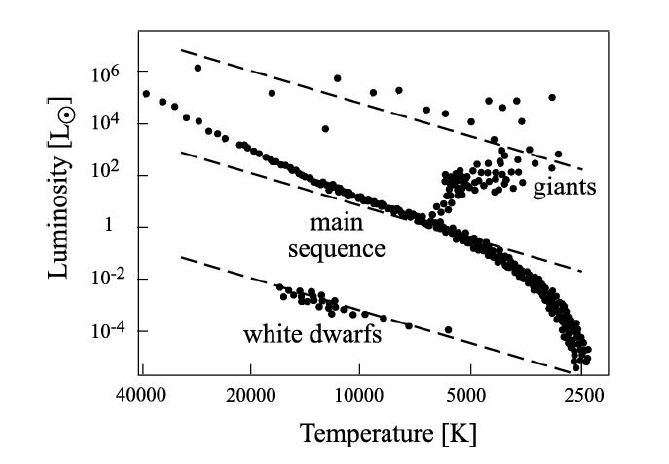
\includegraphics[width=0.7\textwidth]{images/hr-diagram.png}
\end{figure}

\subsection{Stellar Spectral Type}
Stars can be divided into classes based on characteristics.

\begin{figure}[h]
\centering
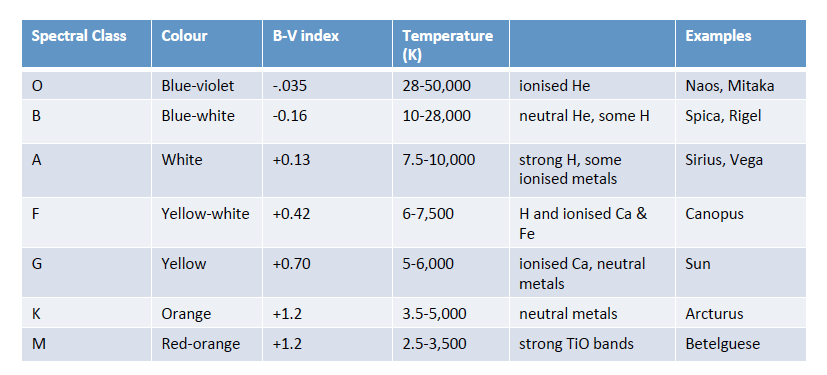
\includegraphics[width=0.7\textwidth]{images/spectral-types.png}
\end{figure}



\pagebreak

%-----------------------------------------
\end{document}







